\documentclass[a4paper,10pt]{article}
\input{/Users/benjamin/Documents/Education/LaTeX/macro.tex}
\usepackage{graphicx}

\title{Architecture �volu�e: S�ance 1}
\author{Benjamin \bsc{Van Ryseghem}}

\begin{document}
\maketitle

\section{Rappel}

\paragraph{ASIC vs. FPGA}
\begin{tabular}{|c|c|c|}
\hline
 & + & - \\
 \hline
 ASIC & performance & prix (premier ~ 10 k\$)\\
 FPGA & prix (~40\$) & performance \\
 \hline
 \end{tabular}

\paragraph{Fichier UCF} Description du circuit, et des liens entre entr�es et sorties.
Chaque ligne sert � mapper un port r�el et un port logique.

\paragraph{D�codeur}
Un d�codeur sert a passer du binaire au d�cimal
Un d�codeur $n$ a $n$ ports en entr�e et $n^2$ ports en sortie.

\section{Exercice 1}
\subsection{Question 1}
Ce syst�me permet l'affichage sur l'afficheur 7 segments l'entr�e lu sur les 4 interrupteurs.
4 interrupteurs binaires fournissent une valeur comprise entre $0$ et $2^4 = 16$. Donc un seul afficheur 4-digits suffit.

\paragraph{Fichier UCF:}
\begin{verbatim}
NET entrees<0> LOC = H13.
NET entrees<1> LOC = H14.
NET entrees<2> LOC = G12.
NET entrees<3> LOC = F12.

NET s7segs<0> LOC = E14.
NET s7segs<1> LOC = G13.
NET s7segs<2> LOC = N15.
NET s7segs<3> LOC = P15.
NET s7segs<4> LOC = R16.
NET s7segs<5> LOC = F13.
NET s7segs<6> LOC = N16.

NET aff<0> LOC = E13.
NET aff<1> LOC = F14.
NET aff<2> LOC = G14.
NET aff<3> LOC = D14.
\end{verbatim}

\subsection{Question 2}
Pour un signal 8bits la valeur en entr�e est comprise entre $0$ et $8^2=256$.

On peut penser a couper les 8bits en 2x4bits. Mais il reste le probl�me de la s�lection de l'afficheur.

Pour cela, on aura besoin d'une horloge (et d'un multiplexeur).
Le multiplexeur peut alors choisir quoi afficher en fonction de l'horloge.

\section{Exercice 2}
\subsection{Question 1}

\begin{figure}[ht]
\begin{center}
     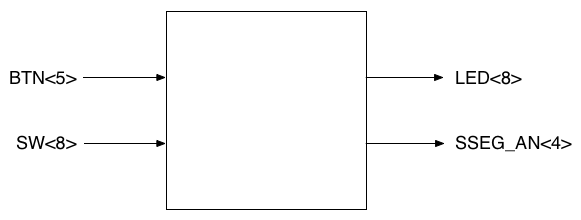
\includegraphics[width=7cm]{figures/ex21.png}
\end{center}
\end{figure}

\subsection{Question 2}
De mani�re g�n�rale, l'ambiguit� n'est pas permise.

\subsection{Question 3}
On cr�e un registre, et on stocke les valeurs.

\section{Exercice 3}
\subsection{Question 1}


\signature

\end{document}